\subsection{Architectural Models}
\subsubsection{UML Deployment Diagram}
In order to ensure good performance and a stable system, the hardware is divided into two layers, internal and external.
The components of the internal system is hosted and maintained by FrostByte, whereas the components of the external system is run by two 3rd parties (ie Visa/Mastercard and TVDB).
\\
Following the diagram is a more in depth explanation of the different components.
\begin{figure}[H]
\fbox{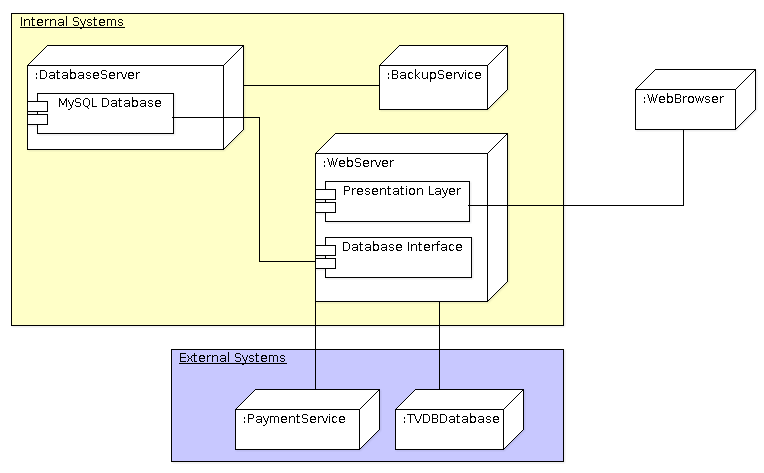
\includegraphics[scale=0.5]{graphics/deployment.png}}
\caption{Deployment Diagram}
\end{figure}

\paragraph*{WebBrowser}~\\
By WebBrowser we are generally talking about the clients, i.e. the users of EpisodeGuide. The clients use a web browser to access data stored on EpisodeGuide through HTTP requests.\\
Supported browsers include Mozilla Firefox, Opera, Chrome and Internet Explorer.

\paragraph*{DatabaseServer}~\\
The database server(s) will store all the available data, including user details, episode information and information about actors. EpisodeGuide will use a graph-oriented database~\cite{website:graphdb}, i.e. a database that uses graph theory to store, map and query relationships. The reason for this is that EpisodeGuide have a lot of data that is linked together, and this could potentialy cause a problem with performance if relational databases and JOIN operations have been used instead.

\paragraph*{WebServer}~\\
The webserver will handle the delivery of data to the clients. Here we have two different components, i.e. the presentation layer and a database interface.\\
The presentation layer provide a way for clients to watch and interact with the content.\\
The database interface is handling the connection(s) to the database(s) and provide a way for the backend to save, modify and delete content.\\
For the database software EpisodeGuide will use the open source NGiNX webserver.

\paragraph*{BackupService}~\\
As a backup service EpisodeGuide will use an encrypted server leveraging the power of RAID-5 with parity bits. Raid-5 will provide a good way to ensure that data is backed up in a safe manner.\\
If a hard drive in this server dies, the use of parity bits will ensure that the lost data can be restored and thus ensuring that no data is lost.\\
Since the database also store information about the clients (i.e. users) the content is fully encrypted using the AES encryption algorithm.

\paragraph*{PaymentService}~\\
\textit{Since this is a 3rd party service, EpisodeGuide has little to no information about the different components or how they are organized.}

\paragraph*{TVDBDatabase}~\\
\textit{Since this is a 3rd party service, EpisodeGuide has little to no information about the different components or how they are organized.}

\subsubsection{User interface flow chart}
\begin{figure}[H]
\fbox{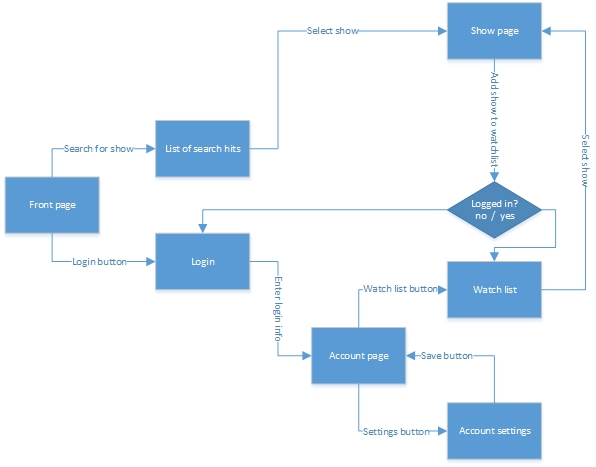
\includegraphics{graphics/UIworkflow}}
\caption{UI flow chart}
\end{figure}

The user interface flow chart is a rough model of the primary functions of the system, and how the end user will navigate through the system. Most of the functions are not modelled and will be implemented around the key features that are modelled. 
